\section{Introduction and Preliminaries}
%
%
%
%
The QUT HPC facilities provide access to,
\begin{itemize}
\item 212 compute nodes
\item 3780 Intel Xeon Cores
\item Approx. 200G B RAM per Compute Nodes
\item 34 TB of main storage
\item 1800 TB additional storage in file store
\item 24 Tesla GPUs
\item Visualisations services and more
\end{itemize}
%
%
%
\subsection{Getting HPC Access}
Before accessing HPC, you will first need to apply for access. This can be done via HiQ by following the instructions on this link \href{https://qutvirtual4.qut.edu.au/group/research-students/doing-your-research/specialty-research-facilities/apply-for-a-hpc-account}{here}. Access will usually be granted in a couple of days at the most.
%
%
\par
%
%
Once access has been granted, you will need a program to access HPC. If you are using a Linux or Mac, you won't need to install anything, though if you are using Windows, it is recommended to use the program PuTTY \cite{putty}. Instructions on logging in to HPC for each OS are given here.
%
%
\subsubsection{Mac and Linux}
To log into HPC, we will be using the Secure SHell (SSH) protocol, which we can access through the command line on Mac and Linux devices. To login, first open a command line prompt (terminal) in your computer. To login, you will need to type in,
\\
\par
\begin{minted}[bgcolor=Light, frame=single, fontsize=\footnotesize, fontfamily=courier]{bash}
  ssh <your_qut_id>@lyra.qut.edu.au
\end{minted}
\\
where you will replace \hltexttt{<your\_qut\_id>} with your QUT username, ie.
\\
\par
\begin{minted}[bgcolor=Light, frame=single, fontsize=\footnotesize, fontfamily=courier]{bash}
  #if you applied for HPC access with staff account
  ssh jane.doe@lyra.qut.edu.au
  #if you applied for HPC access with student account
  ssh n12345678@lyra.qut.edu.au
\end{minted}
%
%
%
%
\subsubsection{Windows}
To login on windows, first install PuTTY by following the instructions \href{https://www.putty.org/}{here}. Once downloaded, open the putty window and enter \hltexttt{lyra.qut.edu.au} into the bar as shown in Figure \ref{fig:putty}. You will then have to enter your QUT username and password.
\begin{figure}[!h]
  \centering
  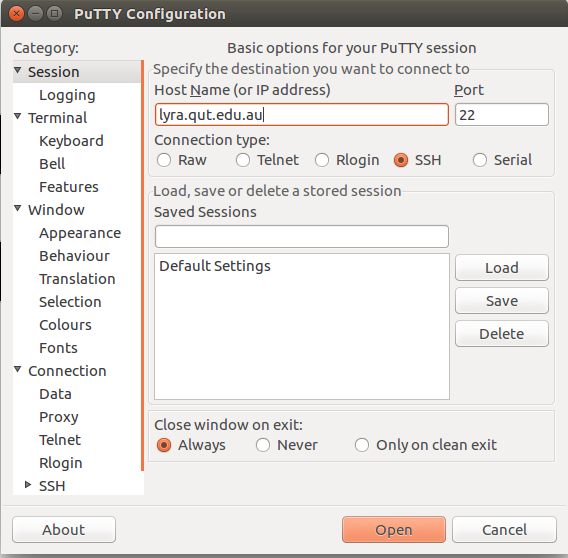
\includegraphics[width=0.5\linewidth]{./figs/putty.png}
  \caption{Example PuTTY window}
  \label{fig:putty}
\end{figure}
%
%
\subsection{Once Logged In}
After following the previous commands you will be logged into the head node of the Lyra HPC cluster. Though you will now be logged in, you have not been allocated any computational resources yet. The head node is available to all users once logged in, and is designed for performing only simple tasks, such as text editing or checking on currently running jobs. If you do start running a program that is computationally expensive, the HPC staff may intervene and kill your process. Running programs from the head node also has the potential to crash the HPC infrastructure. Section \ref{sec:submitting} will explain how to begin submitting jobs using resources you have requested.
%
%
\par
%
%
\subsection{Transferring Files to HPC}
Now that you have access to HPC, you will want to transfer some code over so you can start running some jobs. There are a few ways to do this, though this guide will cover the easier/most prominent ways to do this.
%
%
\par
%
%
To get your code onto HPC, I would recommend using Git and cloning your repo onto HPC. If you are unsure on how to use Git, I would strongly recommend you take some time to learn some basics and start using it for your software projects. Knowledge of Git is not required for this guide, but it will make your software development life significantly better, and allow you to distribute your research much easier.
%
%
\par
%
%
You can clone your repo to HPC via the terminal that is connected to HPC by running the command,
\\
\par
\begin{minted}[bgcolor=Light, frame=single, fontsize=\footnotesize, fontfamily=courier]{bash}
  #change to the home directory
  git clone <remote_url_for_your_repo>
\end{minted}
%
%
\subsection{Mounting HPC Drive on Your Machine}
Directions for how to mount your HPC home drive onto your desktop machine can be found on the \href{https://wiki.qut.edu.au/pages/viewpage.action?pageId=244125273}{QUT HPC Wiki}. The QUT HPC Wiki can be a reasonable source for information, though many of the guides are incomplete, or hard to follow for a new user (hence the creation of this guide!), though the methods for mounting a drive are good. I will provide some alternative methods for mounting a drive here, so feel free to follow either one.
%%
%
%
\subsubsection{Mac and Linux}
It is also helpful to be able to transfer other files to and from HPC. The easiest way to do this is to mount a network directory, so you can copy and paste files to and from HPC just like you would on your desktop/laptop. Instructions on how to do this for Windows, Mac and Linux using SSHFS is provided \href{https://www.digitalocean.com/community/tutorials/how-to-use-sshfs-to-mount-remote-file-systems-over-ssh}{here}. After you install the required programs, you can mount the directory by creating a folder on your desktop where you want to mount your HPC files by running the following command into a terminal that is not logged on to HPC,
%
%
\\
\par
\begin{minted}[bgcolor=Light, frame=single, fontsize=\footnotesize, fontfamily=courier]{bash}
  #run these commands on YOUR MACHINE
  #ie in a new terminal that is not logged on to HPC
  #create a directory on your machine where we will mount the
  #HPC network drive
  mkdir ~/lyra #new folder will be in home directory
  #now mount your HPC home drive to this lyra folder
  #all of this in a single line/command
  sshfs <your_qut_username>@lyra.qut.edu.au:/home/<your_qut_username> ~/lyra
\end{minted}
% 
%
%
\par
\begin{story}
  \textbf{NOTE:}
  \\
  The rest of the commands shown throughout this guide should be run in a terminal that is logged in to HPC
\end{story}
% 
%
\subsubsection{Windows}
For Windows machines, called \href{https://www.nsoftware.com/netdrive/sftp/}{SFTP Net Drive} will allow you to mount your home drive on HPC to your laptop/desktop. After you install the program, type in \hltexttt{lyra.qut.edu.au} as the server, and enter your QUT username and password. This will mount your HPC home drive to your machine in a new drive that can be found in My Computer on your machine.
%
\par
%
An alternative program called \href{https://winscp.net/eng/download.php}{WinSCP} will do allow you transfer files to and from HPC. This is (slightly) less nice to use, but the option is there if you like.
%
%
\subsection{Logging in When Not On QUT's Network}
%
%
Up until now, you would have been required to be at QUT and directly connected to the network to log in to HPC. We can access HPC from off campus by using the \href{https://secure.qut.edu.au/ithelpdesk/qut/softwaredownloads/downloads.jsp}{Cisco Remote Access Client} to open a VPN connection to QUT's network. To open the VPN connection, install the remote client from \ref{https://secure.qut.edu.au/ithelpdesk/qut/softwaredownloads/downloads.jsp}{here}. For the VPN address, use \texttt{sas.qut.edu.au}, then use your QUT staff or student credentials to login. After you have opened the VPN connection, you can log in to HPC using the exact same instructions used previously. This means you can now access HPC from home, from the Botanic Gardens, overseas, or practically anywhere you have an internet connection!
%
%
\par
\begin{story}
  \textbf{NOTE:}
  \\
  You won't be able to open a VPN connection on some networks, such as Eduroam.
\end{story}

%%% Local Variables:
%%% mode: latex
%%% TeX-master: "main"
%%% End: